\chapter{Results}
\label{ch:results}

\section{Lower and upper performance bound}

\section{Grid search for hyperparameters}

% This selects the amount of color to use
% \newcommand*{\MinNumber}{59.1294}%
% \newcommand*{\MaxNumber}{587.674}%

% \newcommand{\ApplyGradient}[1]{%
%     \pgfmathsetmacro{\PercentColor}{100.0*(#1-\MinNumber)/(\MaxNumber-\MinNumber)}
%     \textcolor{black!\PercentColor}{#1}
% }
% \newcolumntype{R}{>{\collectcell\ApplyGradient}{r}<{\endcollectcell}}

\subsection{Full action space}

\begin{figure}[htbp]
    \centering
    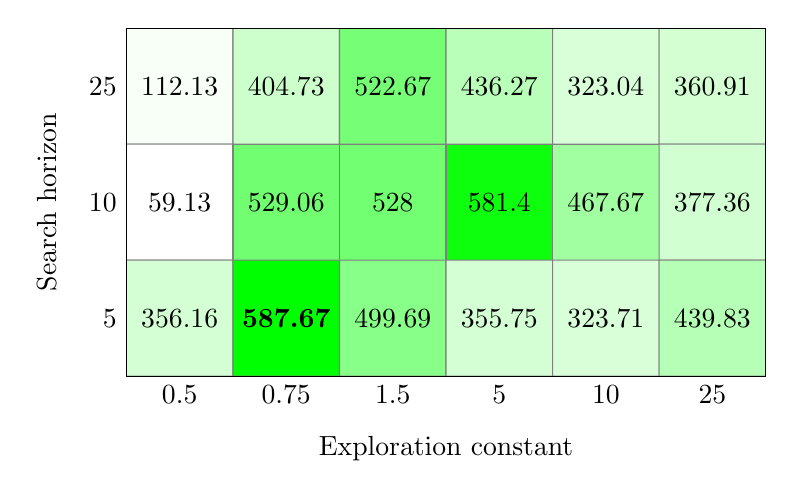
\begin{tikzpicture}
        \begin{axis}[
                width=0.8\linewidth,
                height=6cm,
                colormap={whitegreen}{rgb255(0cm)=(255,255,255); rgb255(4cm)=(204,255,204); rgb255(5.5cm)=(102,255,102); rgb255(6cm)=(0,255,0)},
                xlabel=Exploration constant,
                xlabel style={yshift=-5pt},
                ylabel=Search horizon,
                ylabel style={yshift=5pt},
                xticklabels={0.5, 0.75, 1.5, 5, 10, 25},
                xtick={0,...,5},
                xtick style={draw=none},
                yticklabels={25, 10, 5},
                ytick={0,...,2},
                ytick style={draw=none},
                enlargelimits=false,
                nodes near coords={\ifdim \Cvalue pt = 587.674 pt {\textbf{\pgfmathprintnumber[assume math mode=true]\Cvalue}} \else {\pgfmathprintnumber[assume math mode=true]\Cvalue} \fi},
                visualization depends on={\thisrow{C} \as \Cvalue},
                nodes near coords style={
                    yshift=-7pt
                },
            ]
            \addplot[
                matrix plot,
                mesh/cols=6,
                point meta={\thisrow{C})},
                draw=gray
            ] table {
                x y C
                0 0 112.128
                1 0 404.732
                2 0 522.667
                3 0 436.268
                4 0 323.037
                5 0 360.914
                
                0 1 59.1294
                1 1 529.063
                2 1 528.001
                3 1 581.4
                4 1 467.673
                5 1 377.36
                
                0 2 356.159
                1 2 587.674
                2 2 499.689
                3 2 355.745
                4 2 323.708
                5 2 439.826
            };
        \end{axis}
    \end{tikzpicture}
    \caption{Grid search for the configuration leading to the highest average cumulative reward after 20 runs with up to 1000 actions each, using the full action space.}
\end{figure}

\subsection{Reduced action space}

\begin{figure}[htbp]
    \centering
    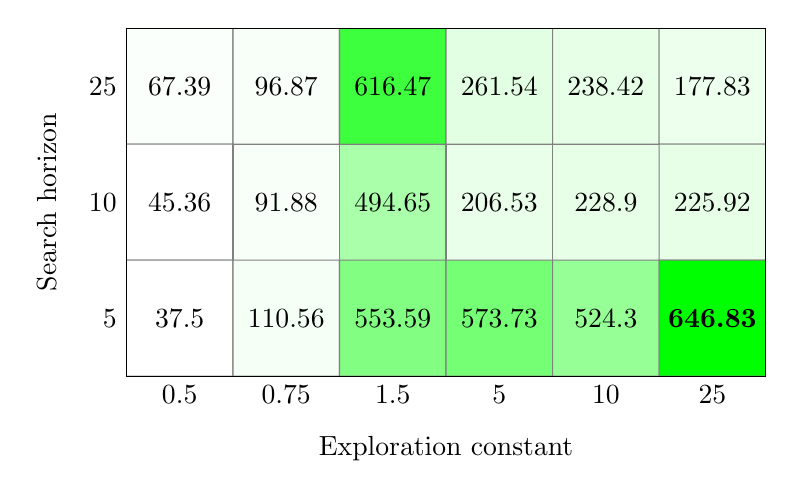
\begin{tikzpicture}
        \begin{axis}[
                width=0.8\linewidth,
                height=6cm,
                colormap={whitegreen}{rgb255(0cm)=(255,255,255); rgb255(4cm)=(204,255,204); rgb255(5.5cm)=(102,255,102); rgb255(6cm)=(0,255,0)},
                xlabel=Exploration constant,
                xlabel style={yshift=-5pt},
                ylabel=Search horizon,
                ylabel style={yshift=5pt},
                xticklabels={0.5, 0.75, 1.5, 5, 10, 25},
                xtick={0,...,5},
                xtick style={draw=none},
                yticklabels={25, 10, 5},
                ytick={0,...,2},
                ytick style={draw=none},
                enlargelimits=false,
                nodes near coords={\ifdim \Cvalue pt = 646.833 pt {\textbf{\pgfmathprintnumber[assume math mode=true]\Cvalue}} \else {\pgfmathprintnumber[assume math mode=true]\Cvalue} \fi},
                visualization depends on={\thisrow{C} \as \Cvalue},
                nodes near coords style={
                    yshift=-7pt
                },
            ]
            \addplot[
                matrix plot,
                mesh/cols=6,
                point meta={\thisrow{C})},
                draw=gray
            ] table {
                x y C
                0 0 67.388
                1 0 96.874
                2 0 616.474
                3 0 261.538
                4 0 238.421
                5 0 177.826
                
                0 1 45.359
                1 1 91.882
                2 1 494.649
                3 1 206.534
                4 1 228.895
                5 1 225.915
                
                0 2 37.504
                1 2 110.563
                2 2 553.591
                3 2 573.726
                4 2 524.302
                5 2 646.833
            };
        \end{axis}
    \end{tikzpicture}
    \caption{Grid search for the configuration leading to the highest average cumulative reward after 20 runs with up to 1000 actions each, using a reduced action space.}
\end{figure}


\subsection{Preferred actions}

\begin{figure}[htbp]
    \centering
    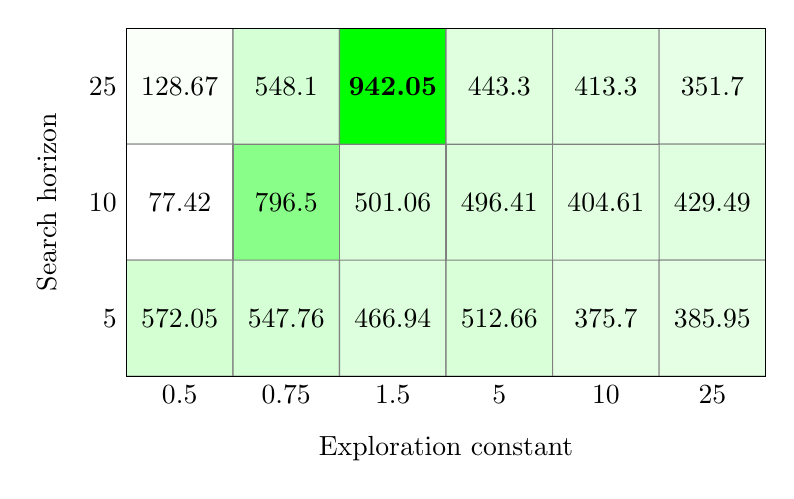
\begin{tikzpicture}
        \begin{axis}[
                width=0.8\linewidth,
                height=6cm,
                colormap={whitegreen}{rgb255(0cm)=(255,255,255); rgb255(4cm)=(204,255,204); rgb255(5.5cm)=(102,255,102); rgb255(6cm)=(0,255,0)},
                xlabel=Exploration constant,
                xlabel style={yshift=-5pt},
                ylabel=Search horizon,
                ylabel style={yshift=5pt},
                xticklabels={0.5, 0.75, 1.5, 5, 10, 25},
                xtick={0,...,5},
                xtick style={draw=none},
                yticklabels={25, 10, 5},
                ytick={0,...,2},
                ytick style={draw=none},
                enlargelimits=false,
                nodes near coords={\ifdim \Cvalue pt = 942.054 pt {\textbf{\pgfmathprintnumber[assume math mode=true]\Cvalue}} \else {\pgfmathprintnumber[assume math mode=true]\Cvalue} \fi},
                visualization depends on={\thisrow{C} \as \Cvalue},
                nodes near coords style={
                    yshift=-7pt
                },
            ]
            \addplot[
                matrix plot,
                mesh/cols=6,
                point meta={\thisrow{C})},
                draw=gray
            ] table {
                x y C
                0 0 128.668
                1 0 548.097
                2 0 942.054
                3 0 443.296
                4 0 413.298
                5 0 351.699
                
                0 1 77.416
                1 1 796.5
                2 1 501.059
                3 1 496.409
                4 1 404.609
                5 1 429.494
                
                0 2 572.054
                1 2 547.758
                2 2 466.936
                3 2 512.66
                4 2 375.698
                5 2 385.954
            };
        \end{axis}
    \end{tikzpicture}
    \caption{Grid search for the configuration leading to the highest average cumulative reward after 20 runs with up to 1000 actions each, using preferred actions.}
\end{figure}

\section{Convergence behavior}

\subsection{Simple driver model}

% TODO: Show how many terminal states were reached

\begin{figure}[htbp]
    \centering
    \begin{tikzpicture}
    \begin{axis}[
        width=\linewidth,
        height=8cm,
        xlabel={Number of searches},
        xtick={10, 100, 200, 300, 400, 500, 750, 1000, 1500, 2500, 5000, 7500, 10000},
        xticklabels={10, 100, 200, 300, 400, 500, 750, 1000, 1500, 2500, 5000, 7500, 10000},
        x tick label style={rotate=60, anchor=east},
        symbolic x coords= {10, 100, 200, 300, 400, 500, 750, 1000, 1500, 2500, 5000, 7500, 10000},
        xmajorgrids=true,
        xminorticks=false,
        ylabel={Average cumulative reward},
        legend pos=south east,
        legend style={font=\small},
        error bars/y dir=both,
        error bars/y explicit
    ]
    \addplot [solid, color=blue, mark=square] table [x=Simulations, y=Average Reward, y error=Standard Error, col sep=comma]{data/Simulations/Simulations - 50 runs - 1000 actions - discount horizon 5 - exp const 0.75 mean.csv};
    \addplot [solid, color=purple, mark=star] table [x=Simulations, y=Average Reward, y error=Standard Error, col sep=comma]{data/Simulations/Reduced Actions - 50 runs - 1000 actions - discount horizon 5 mean.csv};
    \addplot [solid, color=green, mark=diamond] table [x=Simulations, y=Average Reward, y error=Standard Error, col sep=comma]{data/Simulations/Preferred - 50 runs - 1000 actions - discount horizon 25 - exp const 1.5 - reduced mean.csv};
    \addlegendentry{Full action space}
    \addlegendentry{Reduced action space}
    \addlegendentry{Preferred actions}
    \end{axis}
    \end{tikzpicture}
    \caption{Performance comparison of POMCP when utilizing the full action space, a reduced action space, or preferred actions with a simple driver model. Each point shows the mean cumulative reward from 50 runs with 1000 actions each, if no terminal state is reached earlier.}
\end{figure}

\subsection{Steering over-correction}

\begin{figure}[htbp]
    \centering
    \begin{tikzpicture}
    \begin{axis}[
        width=\linewidth,
        height=8cm,
        xlabel={Number of searches},
        xtick={10, 100, 200, 300, 400, 500, 750, 1000, 1500, 2500, 5000, 7500, 10000},
        xticklabels={10, 100, 200, 300, 400, 500, 750, 1000, 1500, 2500, 5000, 7500, 10000},
        x tick label style={rotate=60, anchor=east},
        symbolic x coords= {10, 100, 200, 300, 400, 500, 750, 1000, 1500, 2500, 5000, 7500, 10000},
        xmajorgrids=true,
        xminorticks=false,
        ylabel={Average cumulative reward},
        legend pos=south east,
        legend style={font=\small},
        error bars/y dir=both,
        error bars/y explicit
    ]
    \addplot [solid, color=blue, mark=square] table [x=Simulations, y=Average Reward, y error=Standard Error, col sep=comma]{data/Simulations/Over Correct - 50 runs - 1000 actions - discount horizon 5 mean.csv};
    \addplot [solid, color=purple, mark=star] table [x=Simulations, y=Average Reward, y error=Standard Error, col sep=comma]{data/Simulations/Reduced Actions - Over Correct - 50 runs - 1000 actions - discount horizon 5 mean.csv};
    \addplot [solid, color=green, mark=diamond] table [x=Simulations, y=Average Reward, y error=Standard Error, col sep=comma]{data/Simulations/Preferred - Over Correct - 50 runs - 1000 actions - discount horizon 25 - exp const 1.5 - reduced mean.csv};
    \addlegendentry{Full action space}
    \addlegendentry{Reduced action space}
    \addlegendentry{Preferred actions}
    \end{axis}
    \end{tikzpicture}
    \caption{Performance comparison of POMCP when utilizing the full action space, a reduced action space, or preferred actions with a driver model that over-corrects when it regains attention. Each point shows the mean cumulative reward from 50 runs with 1000 actions each, if no terminal state is reached earlier.}
\end{figure}

\subsection{Steering over-correction and noise}

\begin{figure}[htbp]
    \centering
    \begin{tikzpicture}
    \begin{axis}[
        width=\linewidth,
        height=8cm,
        xlabel={Number of searches},
        xtick={10, 100, 200, 300, 400, 500, 750, 1000, 1500, 2500, 5000, 7500, 10000},
        xticklabels={10, 100, 200, 300, 400, 500, 750, 1000, 1500, 2500, 5000, 7500, 10000},
        x tick label style={rotate=60, anchor=east},
        symbolic x coords= {10, 100, 200, 300, 400, 500, 750, 1000, 1500, 2500, 5000, 7500, 10000},
        xmajorgrids=true,
        xminorticks=false,
        ylabel={Average cumulative reward},
        legend pos=south east,
        legend style={font=\small},
        error bars/y dir=both,
        error bars/y explicit
    ]
    \addplot [solid, color=blue, mark=square] table [x=Simulations, y=Average Reward, y error=Standard Error, col sep=comma]{data/Simulations/Over Correct + Noise - 50 runs - 1000 actions - discount horizon 5 mean.csv};
    \addplot [solid, color=purple, mark=star] table [x=Simulations, y=Average Reward, y error=Standard Error, col sep=comma]{data/Simulations/Reduced Actions - Over Correct + Noise - 50 runs - 1000 actions - discount horizon 5 mean.csv};
    \addplot [solid, color=green, mark=diamond] table [x=Simulations, y=Average Reward, y error=Standard Error, col sep=comma]{data/Simulations/Preferred - Over Correct + Noise - 50 runs - 1000 actions - discount horizon 25 - exp const 1.5 - reduced mean.csv};
    \addlegendentry{Full action space}
    \addlegendentry{Reduced action space}
    \addlegendentry{Preferred actions}
    \end{axis}
    \end{tikzpicture}
    \caption{Performance comparison of POMCP when utilizing the full action space, a reduced action space, or preferred actions with a driver model that over-corrects when it regains attention and performs noisy actions. Each point shows the mean cumulative reward from 50 runs with 1000 actions each, if no terminal state is reached earlier.}
\end{figure}

\section{Comparison of driving trajectories}

% angular jerkiness
% The angular jerkiness is defined as the standard deviation in the change in steering action.

% mean road angle

% mean lane centeredness

\begin{figure}[htbp]
    \centering
    \begin{tikzpicture}
    \begin{axis}[
        width=\linewidth,
        height=8cm,
        xlabel={Number of actions},
        xmajorgrids=true,
        xminorticks=false,
        ylabel={Mean lane centeredness},
        legend pos=south east,
        legend style={font=\small},
        error bars/y dir=both,
        error bars/y explicit
    ]
    \addplot [solid, color=blue, mark=square] table [x=Count, y=Average Distance, y error=Average Distance SE, col sep=comma]{data/Values/Simulations - 50 runs - 1000 actions - discount horizon 5 - exp const 0.75 values.csv};
    \addplot [solid, color=red, mark=star] table [x=Count, y=Average Distance, y error=Average Distance SE, col sep=comma]{data/Values/Reduced Actions - 50 runs - 1000 actions - discount horizon 5 values.csv};
    \addplot [solid, color=green, mark=diamond] table [x=Count, y=Average Distance, y error=Average Distance SE, col sep=comma]{data/Values/Preferred - 50 runs - 1000 actions - discount horizon 25 - exp const 1.5 - reduced values.csv};
    \addlegendentry{1}
    \addlegendentry{2}
    \addlegendentry{3}
    \end{axis}
    \end{tikzpicture}
    \caption{Mean lane centeredness.}
\end{figure}